\documentclass[12pt,a4paper]{article}
\usepackage[UTF8]{ctex}
\usepackage{graphicx}
\usepackage{geometry}
\usepackage{ulem}
\usepackage{enumitem}
\usepackage{titlesec}
\usepackage{multicol}
\usepackage[export]{adjustbox}
\usepackage{amsmath}  % 推荐用于更好的数学排版
\usepackage[utf8]{inputenc}
\usepackage{CJKutf8}
\usepackage{fancyhdr}
\usepackage{lastpage}
\usepackage{ulem}
\usepackage{tabularx}
\usepackage{float}
\usepackage{siunitx}
\usepackage{multirow} 

% 页眉页脚设置
\pagestyle{fancy}
\fancyhf{} % 清除所有页眉页脚
% 设置页眉内容
%-==========1. 填写从第二页开始 每页第一行的信息==========-
\fancyhead[C]{\small
    \makebox[4.5em][c]{实验名称：} \uline{\makebox[17em][c]{集成运算放大器应用电路研究（I）}} 
    \makebox[2.5em][c]{姓名：} \uline{\makebox[4em][c]{}} 
    \makebox[2.5em][c]{学号：} \uline{\makebox[5em][c]{}}
}%--------------------------------------------------------
\fancyfoot[C]{\small 第 \thepage\ 页，共 \pageref{LastPage} 页}


% 取消页眉和页脚的下划线
\renewcommand{\headrulewidth}{0pt} % 页眉横线粗细设为0
\renewcommand{\footrulewidth}{0pt} % 页脚横线粗细设为0

% 调整页眉高度
\setlength{\headheight}{50pt}

% 设置plain样式（用于第一页）
\fancypagestyle{plain}{
    \fancyhf{} % 清除所有页眉页脚
    \renewcommand{\headrulewidth}{0pt} % 隐藏页眉横线
    \fancyfoot[C]{第 \thepage\ 页，共 \pageref{LastPage} 页} % 保留页脚
}
% 设置页面边距
\geometry{left=2.54cm,right=1.5cm,top=2.54cm,bottom=2.54cm}

% 设置正文字体大小为小四
\renewcommand{\normalsize}{\fontsize{12pt}{16pt}\selectfont}
% 设置章节格式
\titleformat{\section}{\fontsize{16pt}{22pt}\selectfont\bfseries}{\thesection}{1em}{} % 一级标题：三号
\titleformat{\subsection}{\fontsize{15pt}{20pt}\selectfont\bfseries}{\thesubsection}{1em}{} % 二级标题：小三

\begin{document}
\thispagestyle{plain}%第一页使用 plain 样式，而不是默认的 fancy 样式，第一页不再显示页眉
% 标题部分 - 两栏布局
\begin{multicols}{2}
    % 左栏：图片和实验报告标题
    % 左栏：使用空行创建前三行
    \noindent
    ~\\ % 第一行
    ~\\ % 第二行
    ~\\ % 第三行
    \hphantom{占位}% 使用空占位符
    \raisebox{-0.5\baselineskip}% 图片向下移动半行
    {
\includegraphics[width=1.85in,height=0.58in]{ZJU.jpg}}
    \hspace{.5em}% 图片和标题之间的间距
    \raisebox{0pt}[\height][0pt]% 标题底部对齐
    {\textbf{\fontsize{26pt}{30pt}\selectfont 实验报告}}
    
    \columnbreak % 换到右栏
    
    % 右栏：个人信息
    % 右栏：个人信息 - 靠右对齐 
%-==========2. 填写个人信息==========-
    \begin{flushright}
        \small
        \makebox[3em][l]{专业：} \uline{\makebox[9em][c]{法语-电子科学与技术}} \\
        \makebox[3em][l]{姓名：} \uline{\makebox[9em][c]{}} \\
        \makebox[3em][l]{学号：} \uline{\makebox[9em][c]{}} \\
        \makebox[3em][l]{日期：} \uline{\makebox[9em][c]{2025年12月16日}} \\
        \makebox[3em][l]{地点：} \uline{\makebox[9em][c]{紫金港东四216}} \\
    \end{flushright}   
\end{multicols}
% 课程名称等信息（单栏）
%-==========3. 填写课程信息==========-

{\small
\noindent
课程名称： \uline{电子电路设计实验I} \hfill 指导老师： \uline{施红军、叶险峰、邓靖靖} \hfill 成绩： \uline{\hspace{3cm}} \\
实验名称：\uline{集成运算放大器应用电路研究（I）}\hfill 实验类型：\uline{设计实验}\hfill 同组学生姓名：\uline{}
}
%-==========4. 正文开始==========-
\section*{一、实验目的}
1、研究由集成运放构成的比例、加法、减法等基本运算电路的组成与功能，加深对集成运放线性应用电路结构和性能特点的理解，掌握其设计方法。

2、研究放大电路增益带宽积与单位增益带宽的关系。

3、了解运算放大器构成的基本运算电路在实际应用时的局限性和应考虑的问题。



\section*{二、实验任务与要求}

\textbf{1、反相放大器设计研究}

(1) 设计一反相放大电路，要求 \( R_i \geq 15\text{k}\Omega \)，\( |A_v| = 15\text{V/V} \)。

(2) 安装该电路，研究输入、输出信号的幅度、相位关系。输入信号幅度合理自定。

\textbf{2、设计并安装一个算术运算电路}

要求实现：\( V_0 = 1.8(V_{i1} - V_{i2}) \)

\( V_{i1} \)用直流、\( V_{i2} \)用正弦信号在合适的幅度和频率范围内，进行验证并记录波形及参数。

\textbf{3、增益带宽积研究}

测量不同增益下的上限频率和增益带宽积。

\section*{三、实验原理}

\subsection*{3.1 理想运算放大器}

在分析或设计集成运放构成的电路时，通常可认为运放是“理想的”。即：

（1）开环差模电压增益 \( A_{ud} = \infty \)

（2）输入电阻 \( R_i = \infty \)
    
（3）输出电阻 \( R_o = 0 \)
    
（4）共模抑制比 \( CMRR = \infty \)
    
（5）带宽 \( BW = \infty \)
    
（6）失调、温漂、内部噪声均为零等。



\subsection*{3.2 理想运放在线性应用时的两个重要特性}

（1） “虚短”：\( U_+ = U_- \)。即运放的同相输入端和反相输入端的电位“无限”接近，就象短路一样，但不是真正的短路。

（2）“虚断”：\( I_+ = 0, I_- = 0 \)。即同相输入端和反相输入端的偏置电流趋于零，就象断路一样，但不是真正的断路。


\subsection*{3.3 基本运算电路}

\subsubsection*{3.3.1 反相放大器（电压并联负反馈）}
\begin{figure}[H]
    \centering
    
\includegraphics[width=0.3\textwidth]{1.png}
    \caption{反相比例放大器电路}
    \label{fig1}
    \end{figure}
放大倍数
\[ 
A_{vf} = \frac{V_o}{V_i} = -\frac{R_F}{R_1}
\]

输入电阻
\[ 
R_i = R_1
\]

输出电阻
\[ 
R_o = 0
\]

其中
\[ 
R_P = R_1 \parallel R_F
\]

\subsubsection*{3.3.2 反相权重加法器}
\begin{figure}[H]
    \centering
    
\includegraphics[width=0.3\textwidth]{2.png}
    \caption{反相权重加法器电路}
    \label{fig2}
    \end{figure}

反相放大器的扩展应用，可以此类推到多个输入信号。                                     
\[
V_o = - \left( \frac{R_F}{R_1} V_{i1} + \frac{R_F}{R_2} V_{i2} \right)\text{，其中}R_P = R_1 \parallel R_2 \parallel R_F
\]

若 \( R_1 = R_2 \)，则
\[
V_o = - \frac{R_F}{R_1} (V_{i1} + V_{i2})
\]

若 \( R_1 = R_2 = R_F \)，则
\[
V_o = - (V_{i1} + V_{i2})
\]

\subsubsection*{3.3.3 同相放大器（电压串联负反馈）}
\begin{figure}[H]
    \centering
    
\includegraphics[width=0.3\textwidth]{3.png}
    \caption{同相放大器电路}
    \label{fig3}
    \end{figure}

\[
A_{vf} = \frac{V_o}{V_i} = 1 + \frac{R_F}{R_1}
\]
\[
R_i = \infty
\]
\[
R_o = 0
\]

若 \( R_1 = \infty \)，则
\[
V_o = V_i
\]
可用来做电压跟随器。

\subsubsection*{3.3.4 差动放大器（减法器）}

\begin{figure}[H]
    \centering
    
\includegraphics[width=0.3\textwidth]{4.png}
    \caption{差动放大器电路}
    \label{fig4}
    \end{figure}
由叠加定理得
\[
V_o = \left( \frac{R_P}{R_2 + R_P} \cdot \frac{R_1 + R_F}{R_1} V_{i2} - \frac{R_F}{R_1} V_{i1} \right)
\]

若电路对称，即\( R_1 = R_2 \)，\( R_F = R_P \)，则
\[
V_o = \frac{R_F}{R_1} (V_{i2} - V_{i1})
\]

\section*{四、实验方案设计与参数计算}

\subsection*{4.1 反相放大器设计}

反相放大器采用如图\ref{fig1}所示的电路，只需要确定参数即可。

设计要求 \( R_i \geq 15\text{k}\Omega \)，\( |A_v| = 15\text{V/V} \)，可得
\[R_i\geq 15\text{k}\Omega,\quad \frac{R_f}{R_1}=15\]

考虑到标称值要求，取
\[R_1=18\text{k}\Omega,\quad R_F=270\text{k}\Omega,\quad R_P=16\text{k}\Omega\]
\subsection*{4.2 算数运算电路设计}

我们要实现的运算，即\( V_0 = 1.8(V_{i1} - V_{i2}) \)，需要使用差分放大器，采用如图\ref{fig4}所示的电路，只需要确定参数即可。但是两个输入需要交换以符合符号的要求。即\(V_{i1}\)对应同相输入端，\(V_{i2}\)对应反相输入端。

由算式可得
\[\frac{R_f}{R_2}=1.8\]

由标称值取
\[R_1=R_2=10\text{k}\Omega,\quad R_F=R_P=18\text{k}\Omega\]

\subsection*{4.3 增益带宽积研究}

采用如下的电路。

\begin{figure}[H]
    \centering
    
\includegraphics[width=0.4\textwidth]{5.png}
    \caption{增益带宽积研究电路}
    \label{fig5}
    \end{figure}

\section*{五、实验仪器设备}

直流稳压电源、信号源、示波器。

\section*{六、实验步骤、调试过程、实验数据记录}

\subsection*{6.1 反相放大器}

输入直流信号，得到如下波形。

\begin{figure}[H]
    \centering
    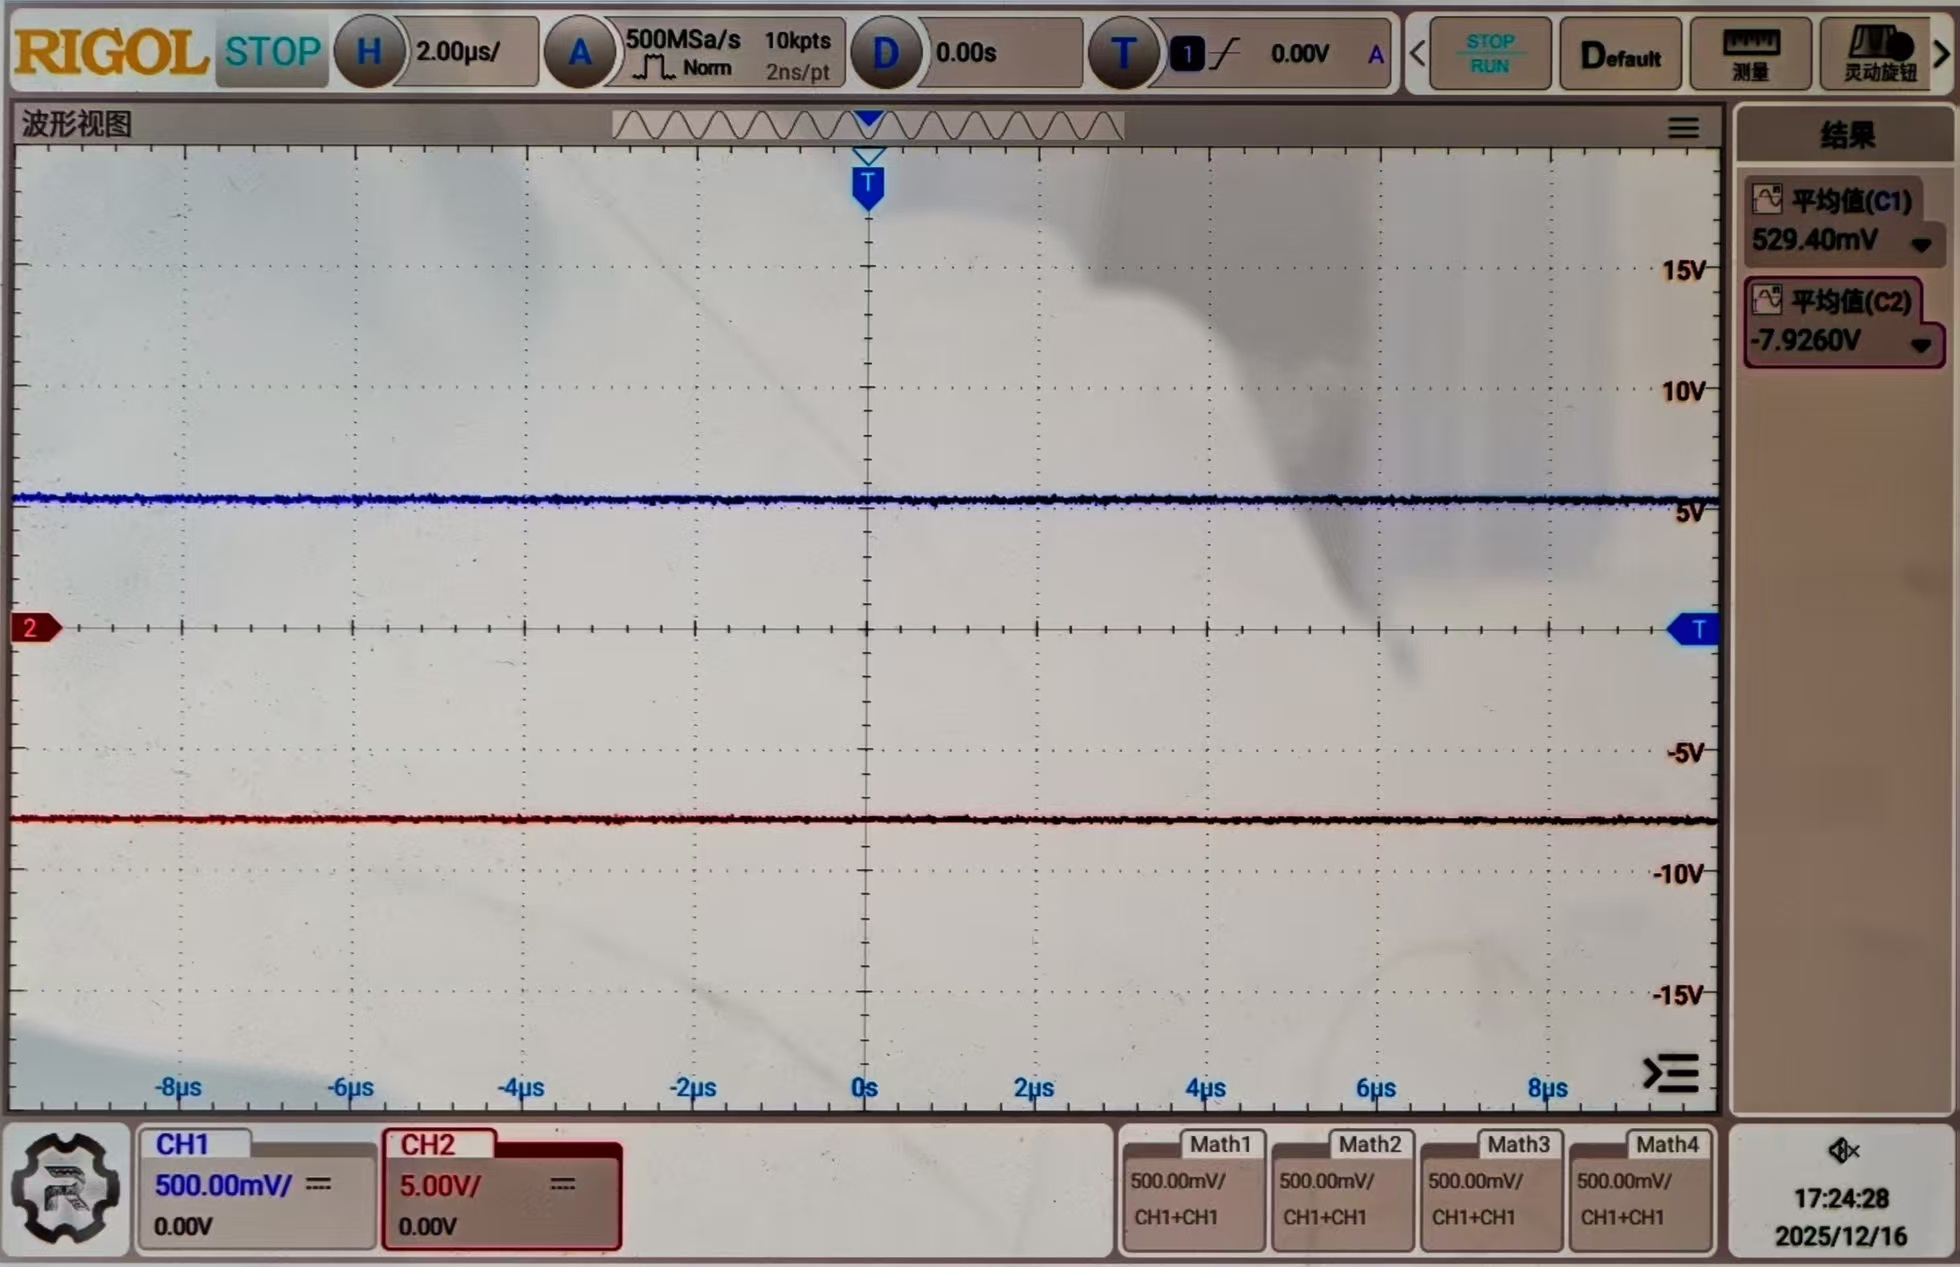
\includegraphics[width=0.8\textwidth]{41.jpg}
    \caption{输入直流信号的波形}
    \label{fig41}
    \end{figure}

输入信号529.4mV，输出信号-7.926V,放大倍数\(A_V=14.97\),说明该电路可以放大直流信号。

输入交流信号，得到如下波形。

\begin{figure}[H]
    \centering
    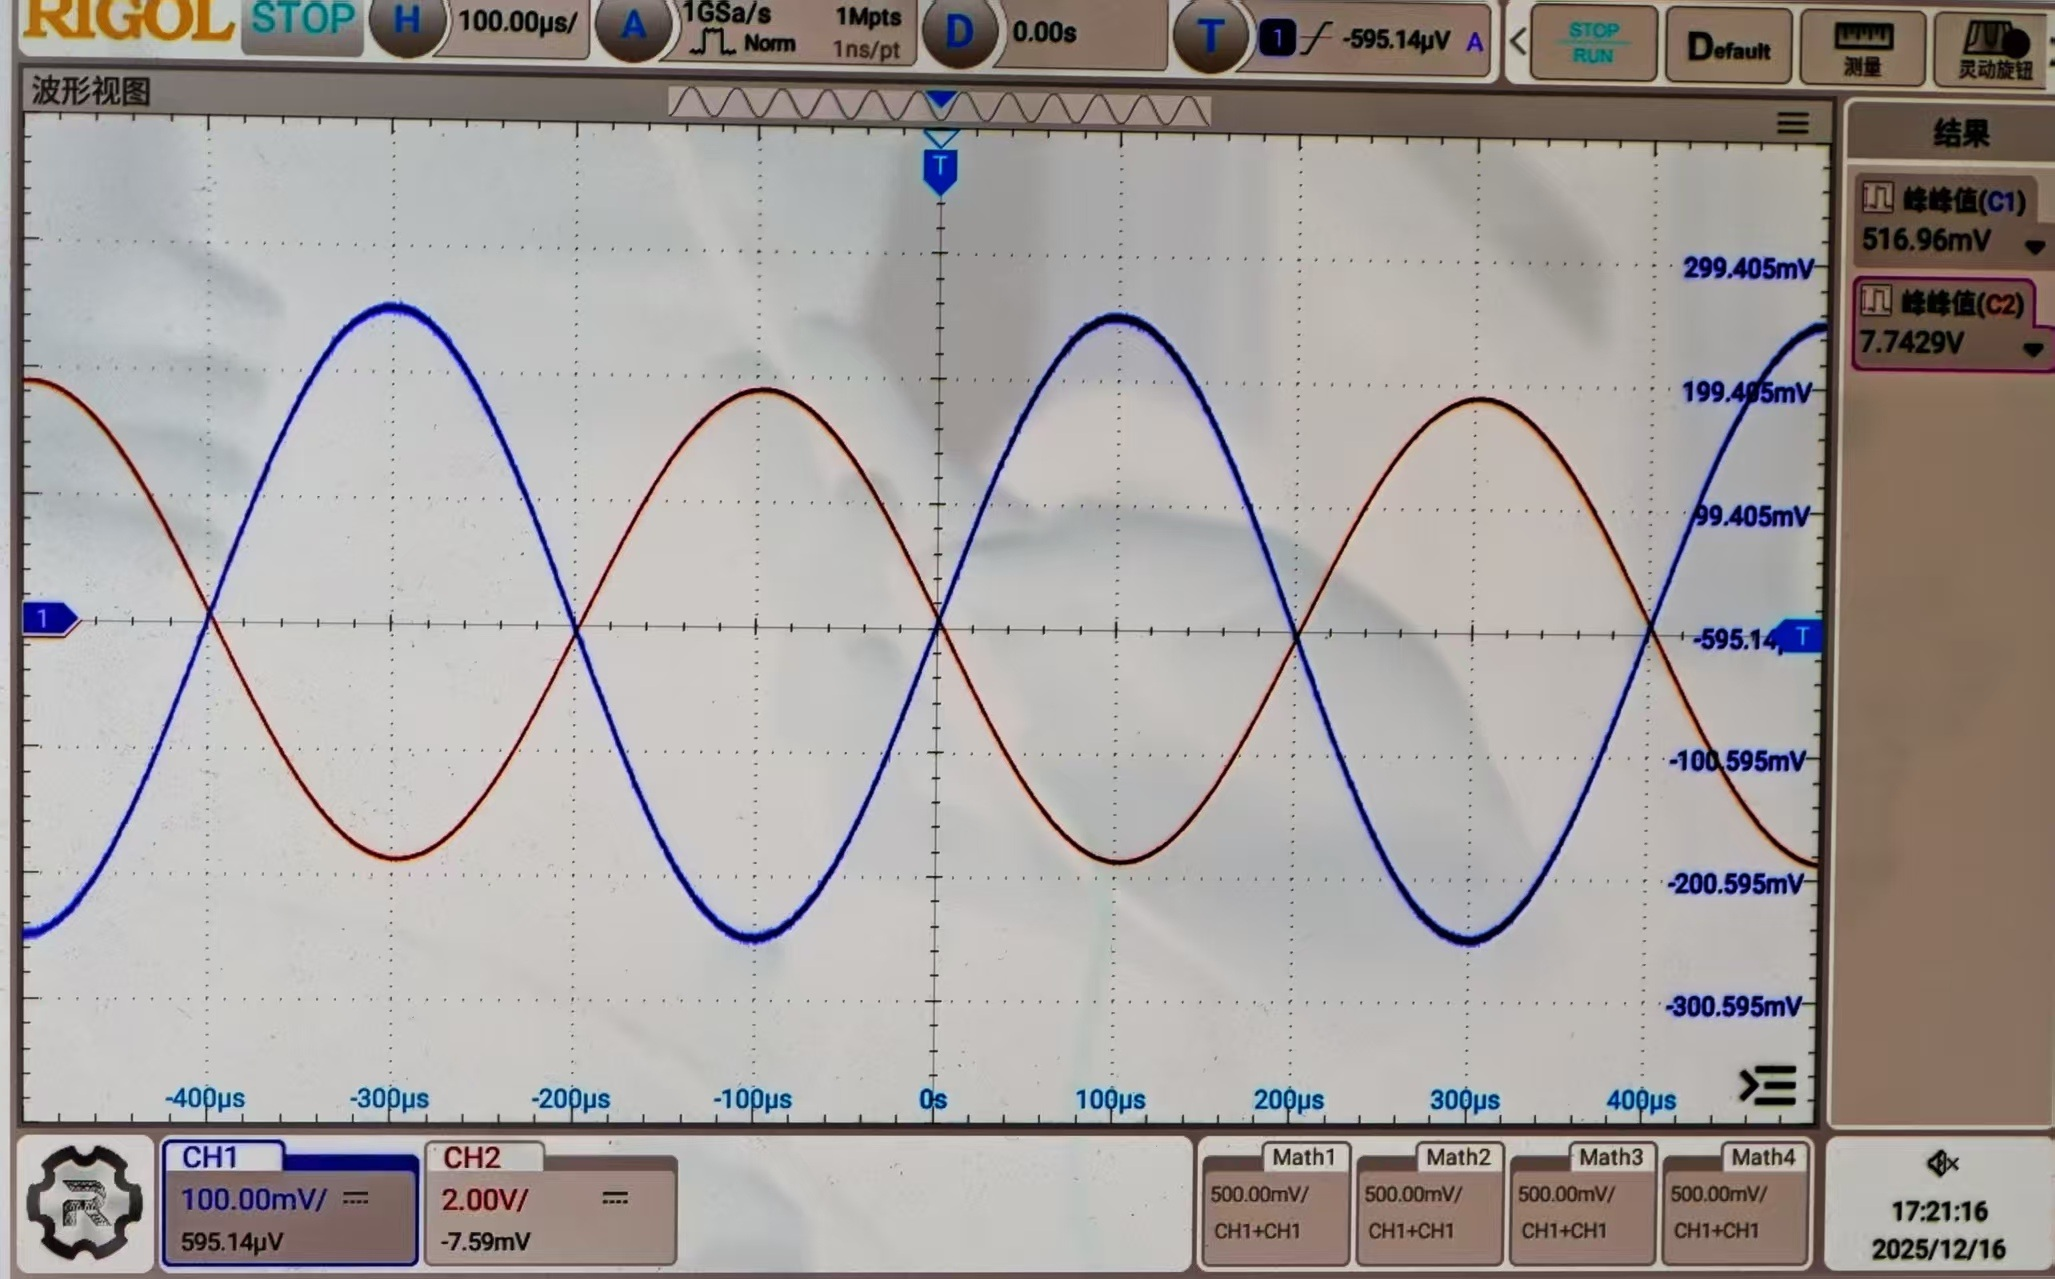
\includegraphics[width=0.8\textwidth]{42.jpg}
    \caption{输入交流信号的波形}
    \label{fig42}
    \end{figure}

输入信号516.96mVpp，输出信号7.7429Vpp,放大倍数\(A_V=14.97\),说明该电路可以放大交流信号。

\subsection*{6.2 算术运算电路}

\(V_{i1}\)输入1.5V直流，\(V_{i2}\)输入3V正弦信号。


在ORCAD中搭建仿真电路，并进行仿真。

\begin{figure}[H]
    \centering
    
\includegraphics[width=0.5\textwidth]{6.png}
    \caption{算术运算电路仿真电路}
    \label{fig6}
    \end{figure}

\begin{figure}[H]
    \centering
    
\includegraphics[width=0.8\textwidth]{7.png}
    \caption{算术运算电路仿真结果}
    \label{fig7}
    \end{figure}

进行实际测量，得到如下波形。

\begin{figure}[H]
    \centering
    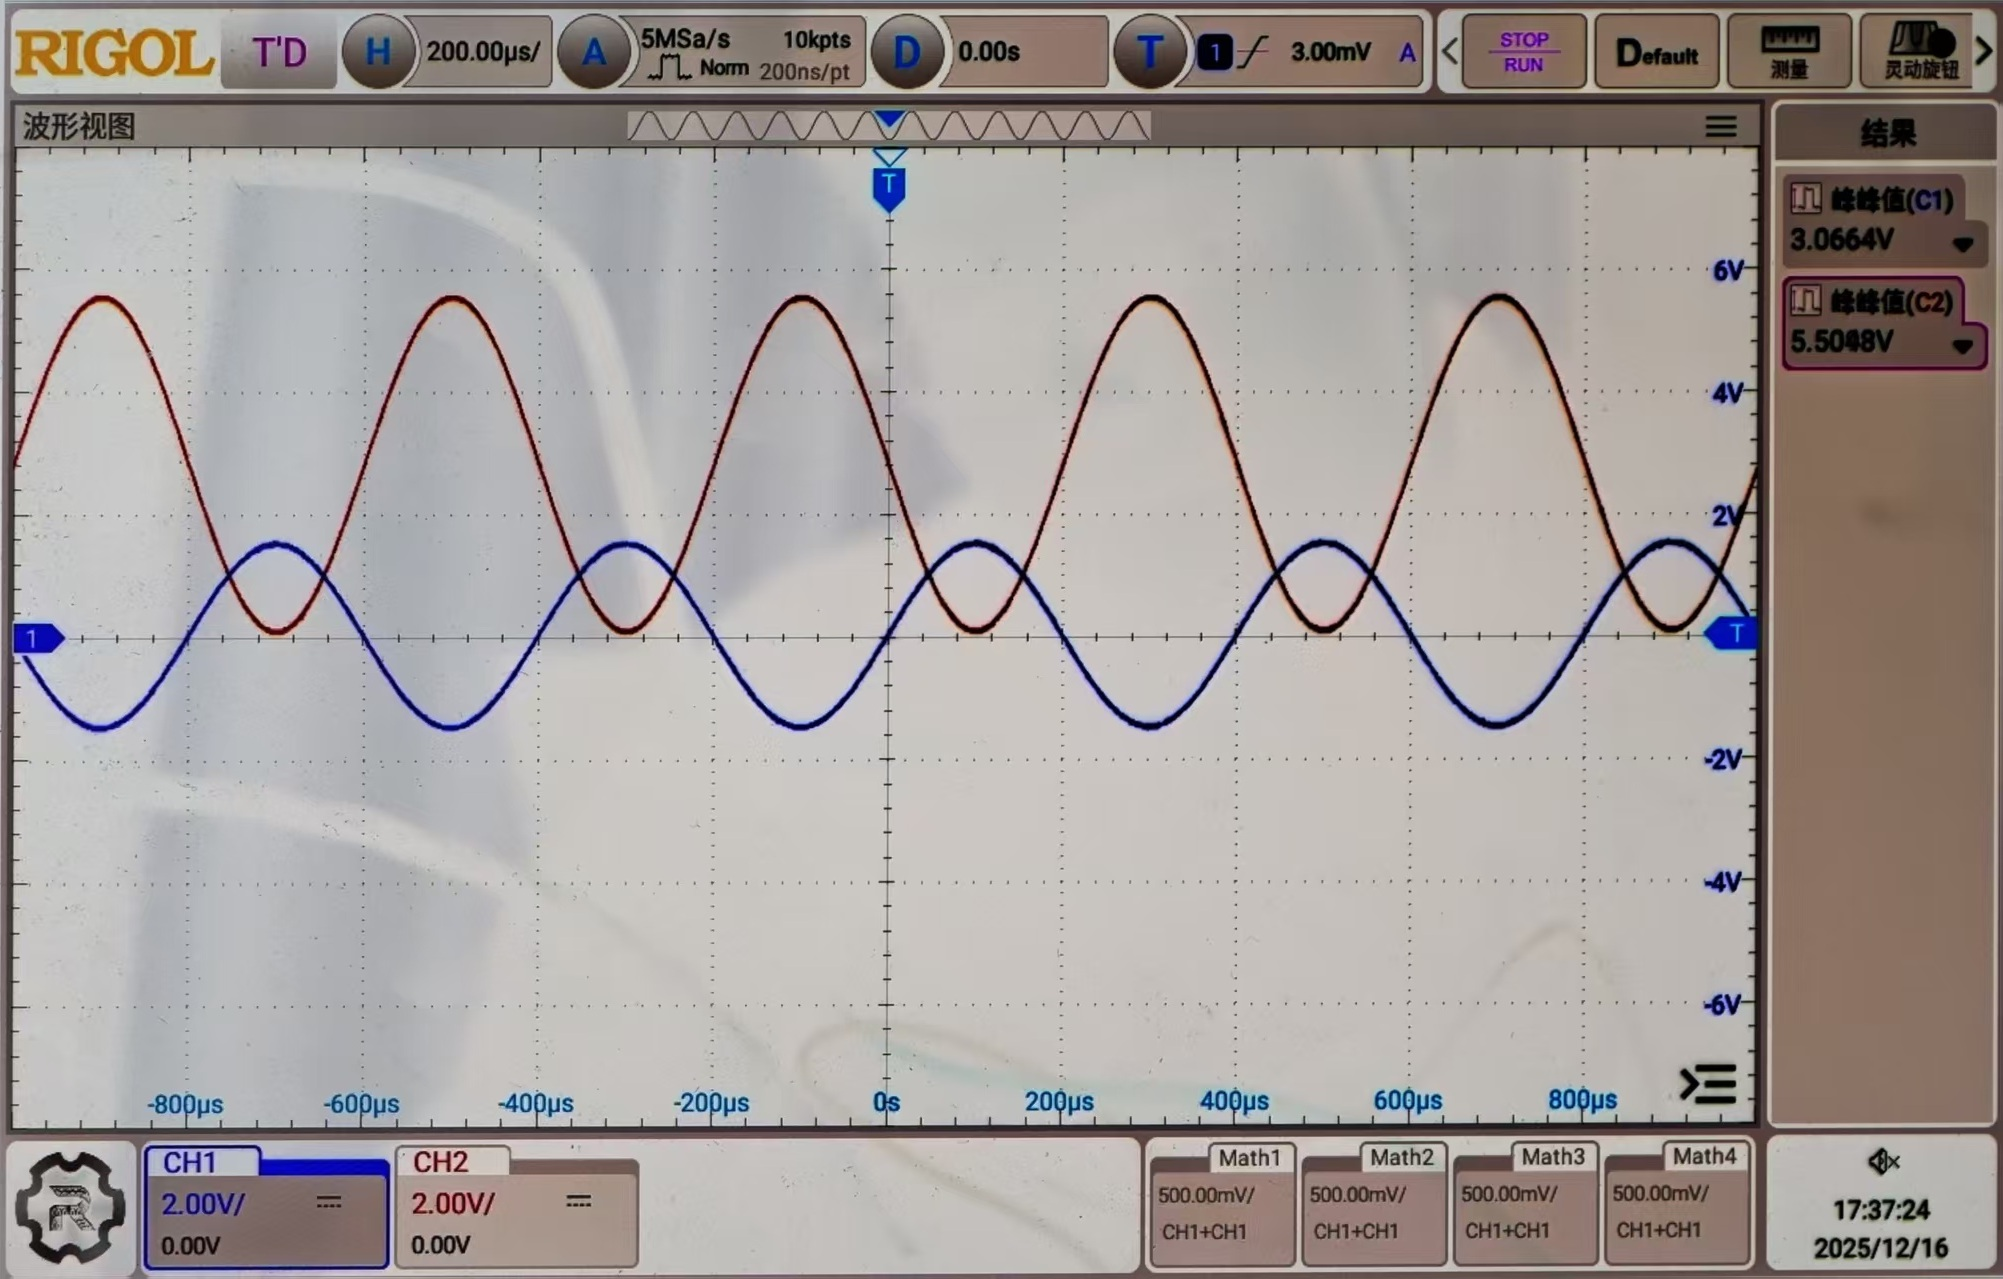
\includegraphics[width=0.8\textwidth]{43.jpg}
    \caption{算术运算电路输出信号波形}
    \label{fig43}
    \end{figure}

可以观察到：

（1）输出信号与输入信号反相，且放大倍数\(A_V=1.796\)。

（2）输出的直流分量为2.84V。

可以说明该电路实现了要求的运算。

\subsection*{6.3 增益带宽积研究}
在ORCAD中搭建仿真电路，并进行仿真。

\begin{figure}[H]
    \centering
    
\includegraphics[width=0.5\textwidth]{9.png}
    \caption{增益带宽积研究仿真电路}
    \label{fig9}
    \end{figure}

\begin{figure}[H]
    \centering
    
\includegraphics[width=0.8\textwidth]{8.png}
    \caption{\(R_f=10\text{k}\Omega\)时的仿真结果}
    \label{fig8}
    \end{figure}

\begin{figure}[H]
    \centering
    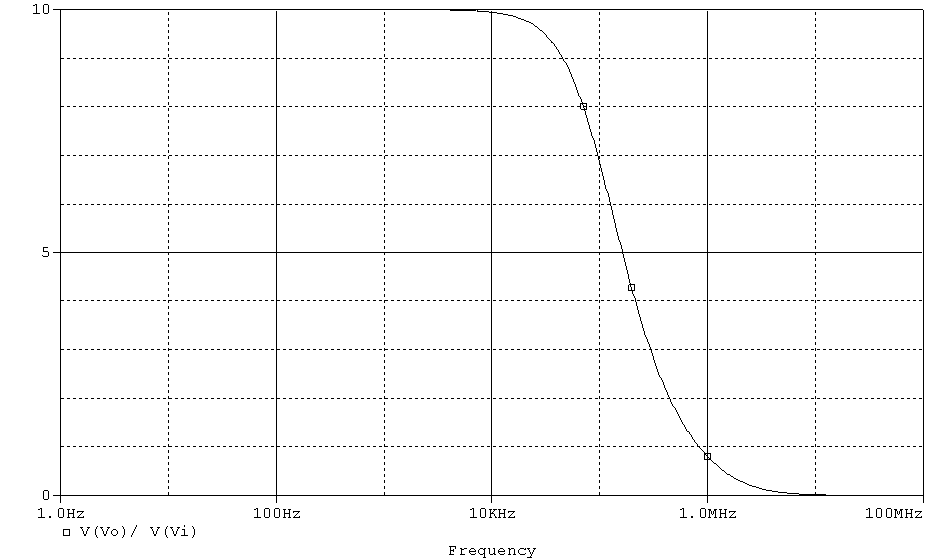
\includegraphics[width=0.8\textwidth]{10.png}
    \caption{\(R_f=100\text{k}\Omega\)时的仿真结果}
    \label{fig10}
    \end{figure}

\begin{figure}[H]
    \centering
    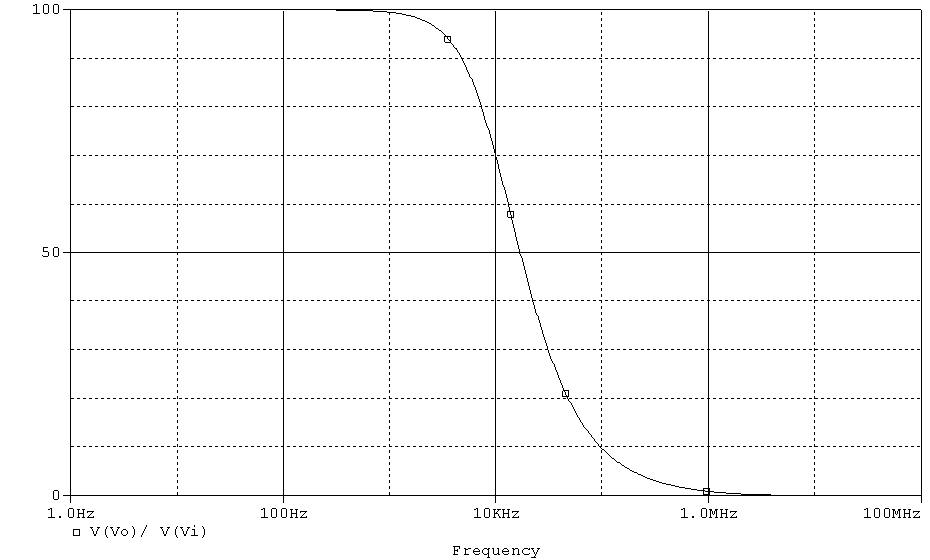
\includegraphics[width=0.8\textwidth]{11.png}
    \caption{\(R_f=1\text{M}\Omega\)时的仿真结果}
    \label{fig11}
    \end{figure}


分别利用光标测出上限频率\(f_h\)。
\begin{table}[h]
    \centering
    \begin{tabular}{|c|c|c|c|c|c|c|c|}
        \hline
        & \( R_1 \) & \( R_f \) & \( R_p \) & \( A_v \) & \( f_H \)(仿真)& \( A_v \cdot BW \)(仿真)  \\
        \hline
        1 & 10 kΩ & 10 kΩ &5.1 kΩ &1  &654.14kHz &654.14kHz \\
        \hline
        2 & 10 kΩ & 100 kΩ &9.1 kΩ &10  &93.80kHz &938.0kHz \\
        \hline
        3 & 10 kΩ & 1 MΩ &10 kΩ &100  &9.79kHz &979.0kHz \\
        \hline
    \end{tabular}
\end{table}



如 \( R_f = 10\ \text{k}\Omega \)，输入幅度 50 mV、频率 1 kHz 正弦信号，增益 \( A_v = 1 \)。保持输入信号幅度不变、逐渐提高频率，开始增益不变。继续提高频率，增益开始下降。直到增益下降到 \( 0.707 A_v \) 时所对应的频率就是增益为 1 时的 \( f_H \)（单位增益带宽）。

更换不同的 \( R_f \) 值，重复上述操作，记录数据。



\begin{table}[h]
    \centering
    \begin{tabular}{|c|c|c|c|c|c|c|}
        \hline
        & \( R_1 \) & \( R_f \) & \( R_p \) & \( A_v \) & \( f_H \)(测量) & \( A_v \cdot BW \)(测量) \\
        \hline
        1 & 10 kΩ & 10 kΩ &5.1 kΩ &1 & 470kHz&470kHz \\
        \hline
        2 & 10 kΩ & 100 kΩ &9.1 kΩ &10 & 75kHz&750kHz \\
        \hline
        3 & 10 kΩ & 1 MΩ &10 kΩ &100 & 7.5kHz&750kHz \\
        \hline
    \end{tabular}
\end{table}








\section*{七、数据分析与讨论}

\subsection*{7.1 反相放大器设计验证}
\begin{itemize}
    \item \textbf{直流输入}：输入529.4 mV，输出-7.926 V，放大倍数 \( A_v = 14.97 \)，与理论值15基本一致，说明电路设计合理，能正常放大直流信号。
    \item \textbf{交流输入}：输入516.96 mVpp，输出7.7429 Vpp，放大倍数 \( A_v = 14.97 \)，相位反相，符合反相放大器特性。
    \item \textbf{结论}：电路满足设计要求，\( R_i = 18k\Omega \geq 15k\Omega \)，增益接近15，误差在合理范围内。
\end{itemize}

\subsection*{7.2 算术运算电路实现}
\begin{itemize}
    \item \textbf{仿真结果}：\( V_0 = 1.796(V_{i1} - V_{i2}) \)，接近理论值1.8，误差较小。
    \item \textbf{实际测量}：
    \begin{itemize}
        \item 输出直流分量为2.84 V，符合 \( V_{i1} = 1.5V \) 直流、\( V_{i2} \) 为3V正弦信号的情况。
        \item 输出波形反相，放大倍数为1.796，验证了差动放大器的功能。
    \end{itemize}
    \item \textbf{讨论}：由于实际电阻值与理论值存在偏差，以及运放本身存在的失调电压等因素，导致放大倍数略有误差，但仍满足设计要求。
\end{itemize}

\subsection*{7.3 增益带宽积研究}
\begin{itemize}
    \item \textbf{仿真与实测对比}：
    \begin{itemize}
        \item 增益带宽积在仿真和实测中均随增益增大而略有变化，但总体上接近常数，符合运放的基本特性。
        \item 实测的 \( f_H \) 普遍低于仿真值，可能与实际运放的带宽限制、寄生电容、测量误差等因素有关。
    \end{itemize}
    \item \textbf{数据趋势}：
    \begin{itemize}
        \item 随着增益 \( A_v \) 增大，\( f_H \) 减小，增益带宽积大致保持恒定，验证了运放的“增益带宽积基本为常数”的特性。
        \item 实测数据中，高增益时（\( A_v = 100 \)）的增益带宽积略低于理论值，可能与运放的频率响应特性有关。
    \end{itemize}
\end{itemize}

\subsection*{7.4 误差来源分析}
\begin{itemize}
    \item \textbf{电阻精度}：实际电阻值与标称值存在偏差，影响放大倍数。
    \item \textbf{运放非理想性}：实际运放存在输入偏置电流、失调电压、有限带宽等非理想因素，尤其在高频下影响显著。
    \item \textbf{测量误差}：示波器读数、信号源输出稳定性等均可能引入误差。
\end{itemize}

\subsection*{7.5 实验设计的合理性}
\begin{itemize}
    \item 所有电路设计均采用标准电路结构，参数选择合理，实验结果与理论吻合度较高。
    \item 通过仿真与实际测量相结合的方式，有效验证了电路功能与性能。
\end{itemize}



\section*{八、结论}

本次实验围绕集成运算放大器的基本应用展开，设计了反相放大器、差动放大器（算术运算电路），并研究了增益带宽积与频率响应的关系。通过理论计算、仿真分析与实际测量相结合的方式，得出以下结论：

\begin{enumerate}
    \item \textbf{反相放大器}：成功设计并实现了 \( R_i = 18k\Omega \)、\( A_v \approx 15 \) 的反相放大电路，输入输出相位相反，放大倍数稳定，符合设计要求。
    \item \textbf{差动放大器（算术运算电路）}：成功实现了 \( V_o = 1.8(V_{i1} - V_{i2}) \) 的运算功能，实测放大倍数 \( A_v \approx 1.796 \)，误差在可接受范围内，验证了差动放大器的减法运算功能。
    \item \textbf{增益带宽积特性}：在不同增益设置下，增益带宽积基本保持恒定，验证了运放的频率响应特性。仿真与实测数据趋势一致，说明电路设计合理，运放性能符合预期。
    \item \textbf{实验方法的有效性}：通过理论计算、仿真验证与实际调试相结合的方法，有效提高了电路设计的准确性与可靠性，加深了对运放线性应用的理解。
\end{enumerate}


\section*{九、心得与体会}

通过本次实验，我获得了以下收获与体会：

\begin{enumerate}
    \item \textbf{理论与实践的结合}：实验让我更直观地理解了运放“虚短”“虚断”的概念，以及反相、同相、差动等基本电路的工作原理。理论计算与实际测量之间的差异，让我认识到元器件非理想性对电路性能的影响。
    \item \textbf{电路设计能力的提升}：从参数选择、仿真验证到实际搭建与调试，我掌握了运放电路的设计流程与调试方法，学会了如何根据设计要求合理选择电阻值，并考虑实际因素进行调整。
    \item \textbf{仿真工具的应用价值}：使用ORCAD进行仿真，能够快速验证电路设计的正确性，预判频率响应等特性，大大提高了实验效率与成功率。
    \item \textbf{误差分析与问题解决能力}：在实验中遇到放大倍数偏差、频率响应不一致等问题时，通过分析误差来源、调整电路参数，提升了问题诊断与解决的能力。
    \item \textbf{团队协作与交流}：与同组同学共同讨论、分工合作，不仅提高了实验效率，也增强了沟通与协作能力。
\end{enumerate}

总之，本次实验不仅巩固了课堂所学知识，也锻炼了我的动手能力与工程思维，为后续深入学习电子电路设计奠定了基础。



\end{document}